\documentclass[10pt,aspectratio=43,mathserif,table]{beamer} 
%设置为 Beamer 文档类型,设置字体为 10pt,长宽比为16:9,数学字体为 serif 风格
\batchmode

\usepackage{graphicx}
\usepackage{animate}
\usepackage{hyperref}

%导入一些用到的宏包
\usepackage{amsmath,bm,amsfonts,amssymb,enumerate,epsfig,bbm,calc,color,ifthen,capt-of,multimedia,hyperref}
\usepackage{xeCJK} %导入中文包
\setCJKmainfont{SimHei} %字体采用黑体  Microsoft YaHei

\usetheme{Goettingen} %主题
%\usecolortheme{sustech} %主题颜色

\usepackage[ruled,linesnumbered]{algorithm2e}

\usepackage{fancybox}
\usepackage{xcolor}
\usepackage{times}
\usepackage{listings}

\usepackage{booktabs}
\usepackage{colortbl}

\newcommand{\Console}{Console}
\lstset{ %
	backgroundcolor=\color{white},   % choose the background color
	basicstyle=\footnotesize\rmfamily,     % size of fonts used for the code
	columns=fullflexible,
	breaklines=true,                 % automatic line breaking only at whitespace
	captionpos=b,                    % sets the caption-position to bottom
	tabsize=4,
	commentstyle=\color{mygreen},    % comment style
	escapeinside={\%*}{*)},          % if you want to add LaTeX within your code
	keywordstyle=\color{blue},       % keyword style
	stringstyle=\color{mymauve}\ttfamily,     % string literal style
	numbers=left, 
	%	frame=single,
	rulesepcolor=\color{red!20!green!20!blue!20},
	% identifierstyle=\color{red},
	language=c
}

\setsansfont{Microsoft YaHei}
\setmainfont{Microsoft YaHei}

\definecolor{mygreen}{rgb}{0,0.6,0}
\definecolor{mymauve}{rgb}{0.58,0,0.82}
\definecolor{mygray}{gray}{.9}
\definecolor{mypink}{rgb}{.99,.91,.95}
\definecolor{mycyan}{cmyk}{.3,0,0,0}

%题目,作者,学校,日期
\title{The China Syndrome}
\subtitle{\fontsize{9pt}{14pt}\textbf{local labor market effects of import competition in the United States}}
\author{Author: David H. Autor; David Dorn; Gordon H. Hanson \newline \newline Reported by:MENG Ke }
\institute{\fontsize{8pt}{14pt}China Institute for WTO Studies, UIBE}
\date{\today}

%学校Logo
%\pgfdeclareimage[height=0.5cm]{sustech-logo}{sustech-logo.png}
%\logo{\pgfuseimage{sustech-logo}\hspace*{0.3cm}}

\AtBeginSection[]
{
	\begin{frame}<beamer>
	\frametitle{\textbf{Content}}
	\tableofcontents[currentsection]
\end{frame}
}
\beamerdefaultoverlayspecification{<+->}
% -----------------------------------------------------------------------------
\begin{document}
% -----------------------------------------------------------------------------

\frame{\titlepage}

\section[Content]{}   %目录
\begin{frame}{Content}
\tableofcontents
\end{frame}

% -----------------------------------------------------------------------------
\section{Introduction}  %引言
\subsection{Conclusion}
\begin{frame}{Conclusion}
	Main conclusions of this paper:
	\begin{block}{conclusion}
		\begin{itemize}
			\item<0->  The EXPOSURE to Chinese import competition affects US local labor markets
			\item<0->  The rising EXPOSURE increase unemployment, lowers labor force participation and reduces wages in local labor market.
			\item<0->  This effect explains 1/4 of the contemporaneous aggregate decline in U.S. manufacturing employment.
		\end{itemize}
	\end{block}
\end{frame}
\subsection{Background}
\begin{frame}{Background}
	%\begin{block}{Background}
		\begin{itemize}
			\item<0->  After China's accession to the WTO, its economic growth has been impressive, China's exports to the world increase at a skyrocked way.
			\item<0->  Unequal wages in the U.S. labor market, rising unemployment in manufacturing.
			\item<0->  The share of total U.S. spending on Chinese goods rose from 0.6\% in 1991 to 4.6\% in 2007.
		\end{itemize}
	%\end{block}
\end{frame}
\begin{frame}{Background}
	\begin{figure}[thpb]
		\centering
		\resizebox{1\linewidth}{!}{
			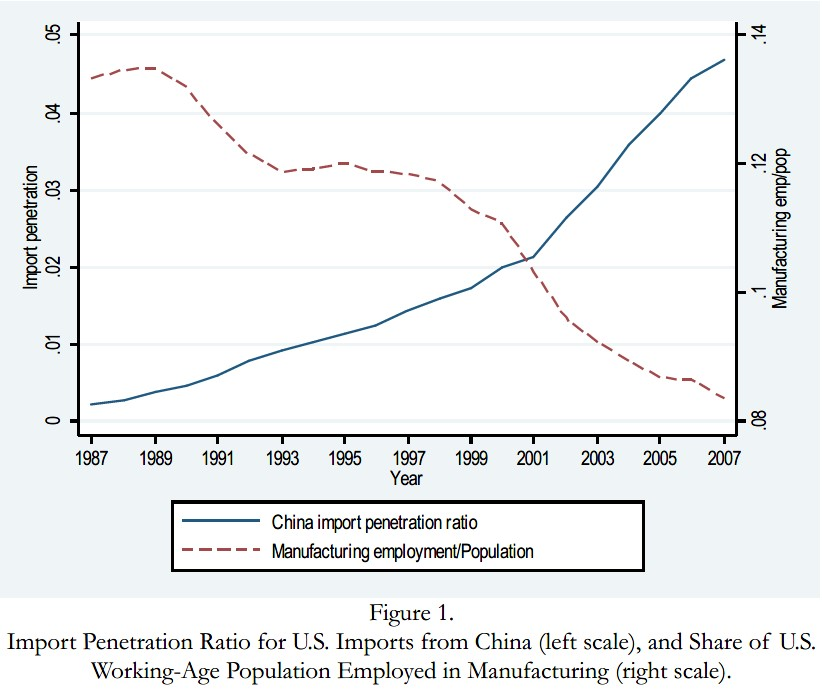
\includegraphics{figures/fig1.jpg}
		}
		%\includegraphics[scale=1.0]{figurefile}
		%\caption{Fig1}
		%\label{fig:campus}
	\end{figure}
\end{frame}

\begin{frame}{Data}
	\centering
	\resizebox{1\linewidth}{!}{
		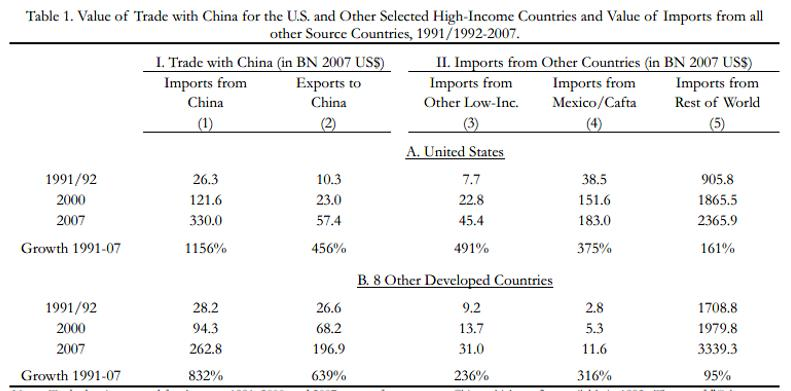
\includegraphics{figures/table1.jpg}
	}
	%\includegraphics[scale=1.0]{figurefile}
	%\caption{Fig1}
	%\label{fig:campus}	
\end{frame}

\subsection{A Shift-Share Method}
\begin{frame}{Shift-Share}
\alert{QUESTION: What is EXPOSURE?}
\begin{block}{Shift-share:	Consider regional economic changes as a dynamic process}

\begin{center}
	\Large $\Delta IPW_{uit}=\sum_{j} \frac{L_{ijt}}{L_{it}} \frac{\Delta M_{ucjt}}{L_{ujt}} $
    \\[5mm]
	\Large $\Delta IPW_{oit}=\sum_{j} \frac{L_{ijt-1}}{L_{it-1}} \frac{\Delta M_{ocjt}}{L_{ujt-1}} $
\end{center}
	\textit{i:region \qquad j:industry \qquad t:time \\  M:import from China \quad L:employment}
\end{block}
\end{frame}





\section{Data Sources \&measurement}  

\begin{frame}{Data}
	\begin{itemize}
		\item<0->  Export:from UN comtrade (HS6 digit)
		\item<0->  Employment:Employment data for 397 manufacturing industries comes from County Business Patterns data
		\item<0->  US regional(i):Commuting Zones (CZs) 
	\end{itemize}

\end{frame}
\begin{frame}{Data}
		\centering
\resizebox{1\linewidth}{!}{
	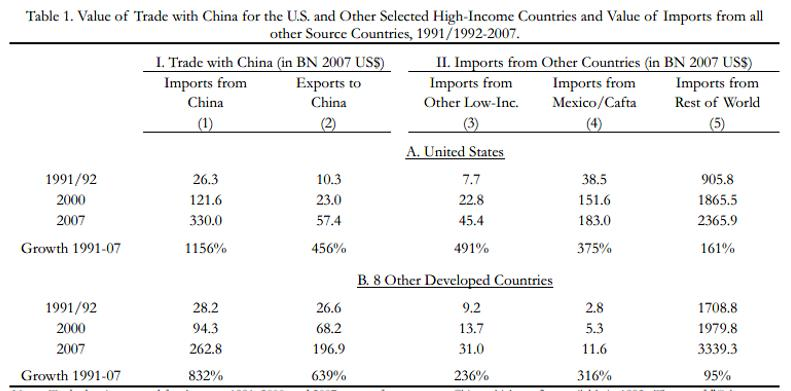
\includegraphics{figures/table1.jpg}
}
%\includegraphics[scale=1.0]{figurefile}
%\caption{Fig1}
%\label{fig:campus}	
\end{frame}

\begin{frame}{Data}
	\begin{itemize}
		\item<0->  Export:from UN comtrade (HS6 digit)
		\item<0->  Employment:Employment data for 397 manufacturing industries comes from County Business Patterns data
		\item<0->  US regional(i):Commuting Zones (CZs) 
	\end{itemize}
	
\end{frame}


\begin{frame}{X:exposure}
	\centering
	\resizebox{1\linewidth}{!}{
		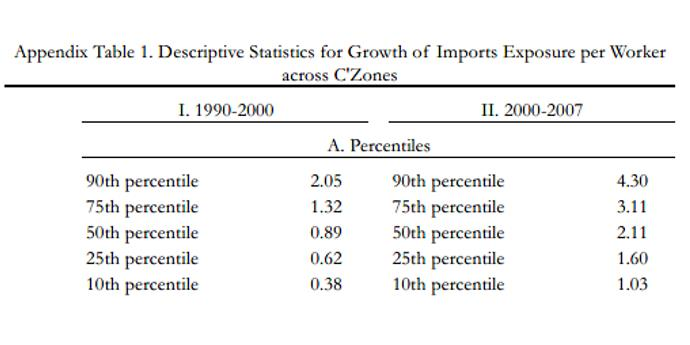
\includegraphics{figures/Atable1.jpg}
	}
	%\includegraphics[scale=1.0]{figurefile}
	%\caption{Fig1}
%	\label{fig:campus}	
\end{frame}


\begin{frame}{X:exposure}
	\centering
	\resizebox{1\linewidth}{!}{
		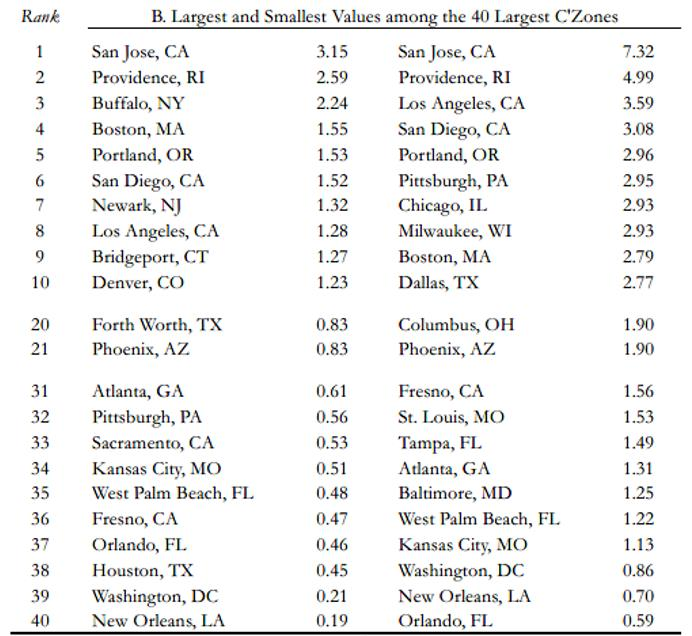
\includegraphics{figures/Atable2.jpg}
	}
	%\includegraphics[scale=1.0]{figurefile}
	%\caption{Fig1}
%	\label{fig:campus}	
\end{frame}



\begin{frame}{Y:dependent variable}
	\centering
	\resizebox{1\linewidth}{!}{
		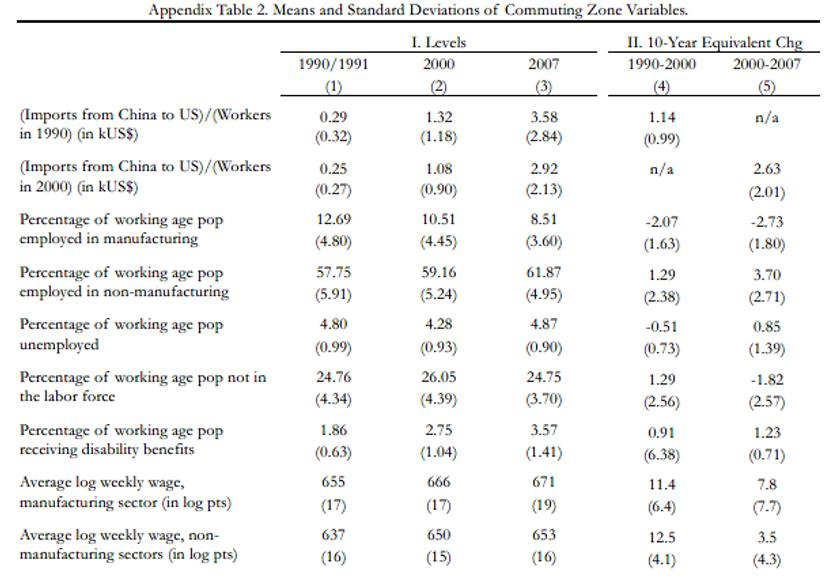
\includegraphics{figures/Atable3.jpg}
	}
	%\includegraphics[scale=1.0]{figurefile}
	%\caption{Fig1}
%	\label{fig:campus}	
\end{frame}




\begin{frame}{Y:dependent variable}
	\centering
	\resizebox{1\linewidth}{!}{
		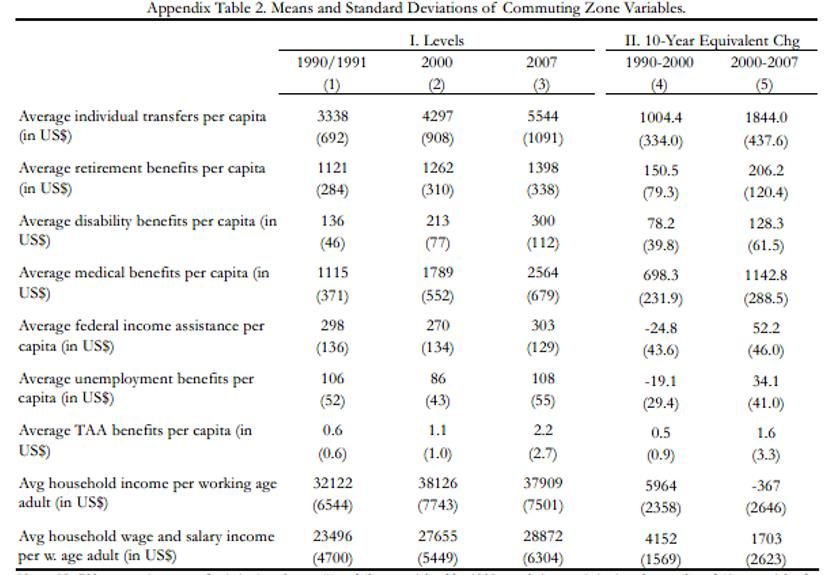
\includegraphics{figures/Atable4.jpg}
	}
	%\includegraphics[scale=1.0]{figurefile}
	%\caption{Fig1}
%	\label{fig:campus}	
\end{frame}




\section{Empirical approach}
\subsection{IV Strategy}
\begin{frame}{instrumental variable strategy}
	\begin{center}
		\Large $\Delta IPW_{uit}=\sum_{j} \frac{L_{ijt}}{L_{ujt}} \frac{\Delta M_{ucjt}}{L_{it}} $     (1)
		\\[5mm]
		\Large $\Delta IPW_{oit}=\sum_{j} \frac{L_{ijt-1}}{L_{ujt-1}} \frac{\Delta M_{ocjt}}{L_{it-1}} $   (2)
	\end{center}
	\begin{itemize}
		\item<0-> Endogeneity: U.S. imports from China in (1) may be correlated with industry labor demand shocks.
		\item<0-> employ an instrumental variables using the exogenous component of Chinese imports.
		\item<0-> using data on contemporaneous industry-level growth of Chinese exports to other high-income markets; Build exposure as shown in (2)
	\end{itemize}
\end{frame}

\begin{frame}{instrumental variable strategy}
	\begin{center}
		\Large $\Delta L^{m}_{it}=\gamma_{t} + \beta_{1} \Delta IPW_{uit} + X^{`}_{it} \beta_{2} + e_{ct}  $     

	\end{center}
\begin{figure}[thpb]
	\centering
	\resizebox{1\linewidth}{!}{
		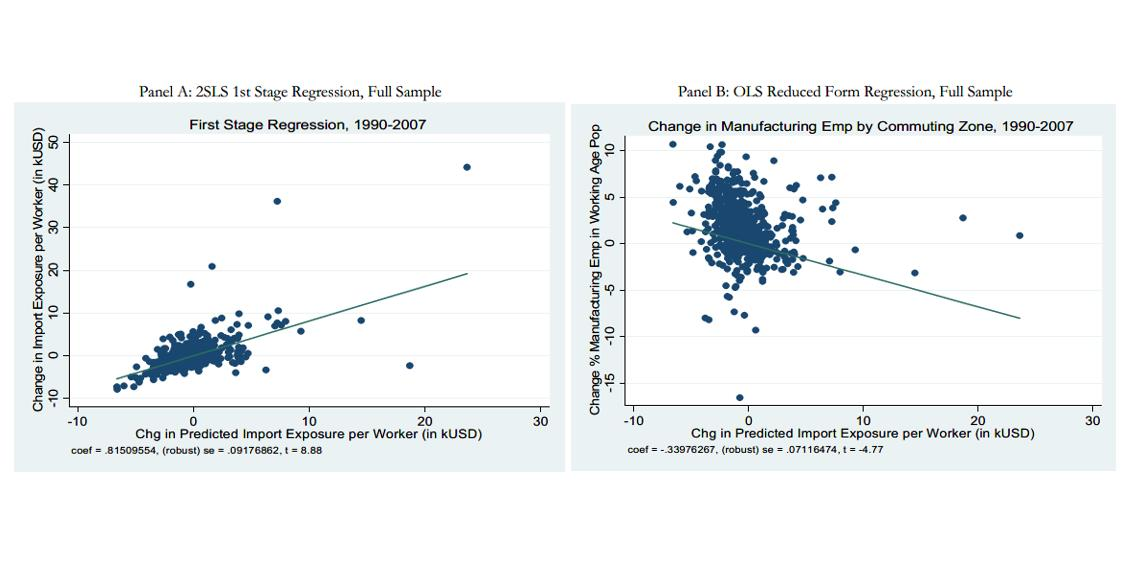
\includegraphics{figures/fig2.jpg}
	}
	%\includegraphics[scale=1.0]{figurefile}
	%\caption{Fig1}
%	\label{fig:campus}
\end{figure}
\end{frame}

\subsection{Result}
\begin{frame}{Result}
	\begin{center}
		\Large $\Delta L^{m}_{it}=\gamma_{t} + \beta_{1} \Delta IPW_{uit} + X^{`}_{it} \beta_{2} + e_{ct}  $     
		
	\end{center}
	\begin{figure}[thpb]
		\centering
		\resizebox{1\linewidth}{!}{
			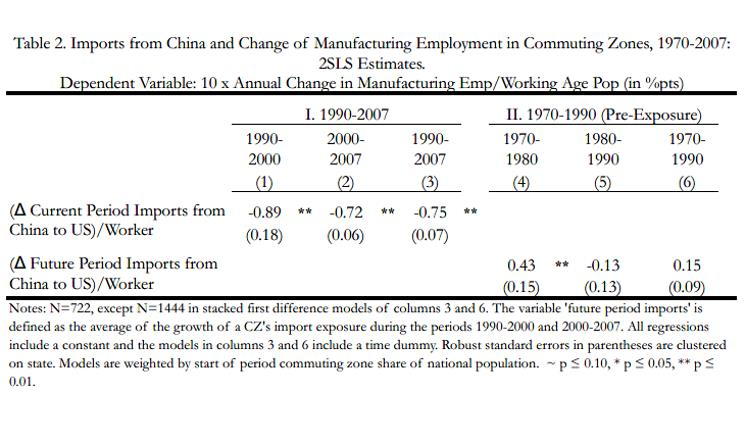
\includegraphics{figures/table2.jpg}
		}
		%\includegraphics[scale=1.0]{figurefile}
		%\caption{Fig1}
%		\label{fig:campus}
	\end{figure}
\end{frame}

\begin{frame}{Result}
	\begin{figure}[thpb]
		\centering
		\resizebox{1\linewidth}{!}{
			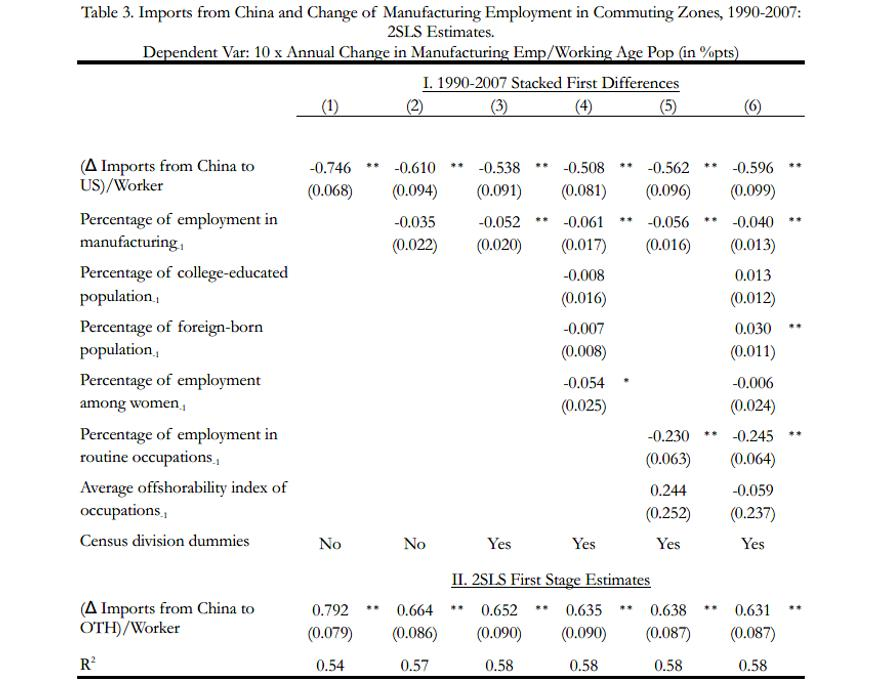
\includegraphics{figures/table3.jpg}
		}
		%\includegraphics[scale=1.0]{figurefile}
		%\caption{Fig1}
%		\label{fig:campus}
	\end{figure}
\end{frame}


\section{Beyond manufacturing}
\subsection{population effect}
\begin{frame}{population effect}
	\begin{figure}[thpb]
		\centering
		\resizebox{1\linewidth}{!}{
			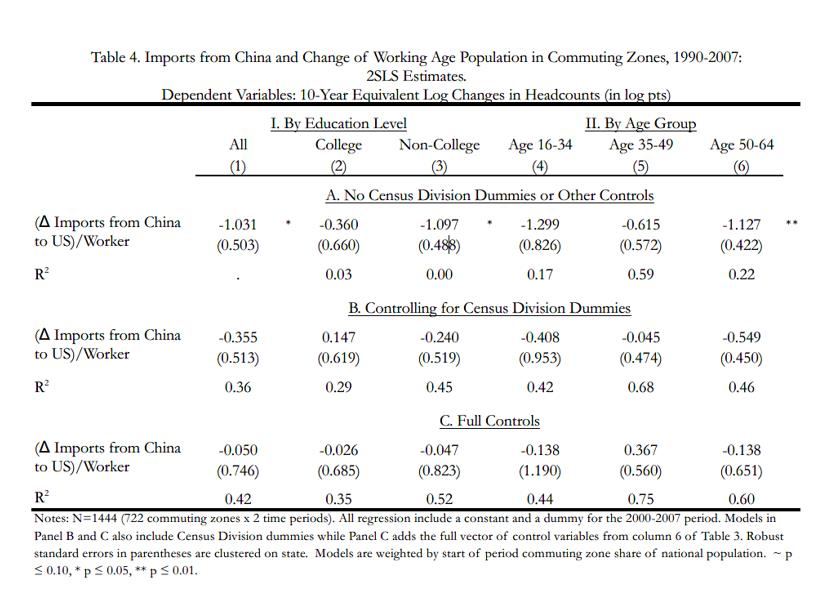
\includegraphics{figures/table4.jpg}
		}
		%\includegraphics[scale=1.0]{figurefile}
		%\caption{Fig1}
%		\label{fig:campus}
	\end{figure}
\end{frame}

\subsection{employmet effect}
\begin{frame}{employmet effect}
	\begin{figure}[thpb]
		\centering
		\resizebox{1\linewidth}{!}{
			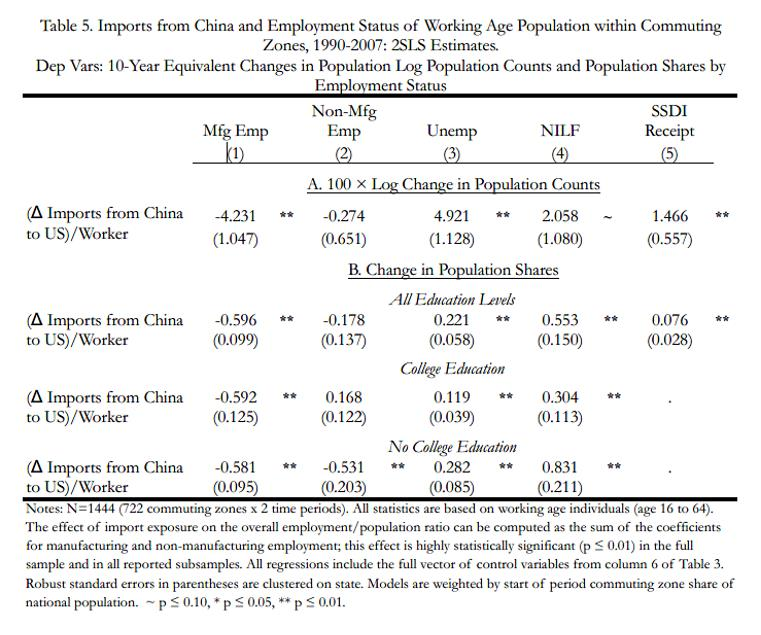
\includegraphics{figures/table5.jpg}
		}
		%\includegraphics[scale=1.0]{figurefile}
		%\caption{Fig1}
%		\label{fig:campus}
	\end{figure}
\end{frame}

\subsection{Wage effect}
\begin{frame}{Wage effect}
	\begin{figure}[thpb]
		\centering
		\resizebox{1\linewidth}{!}{
			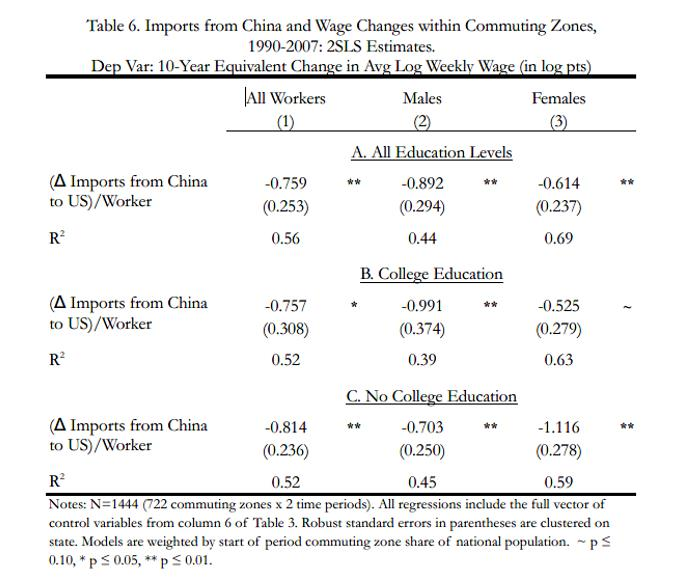
\includegraphics{figures/table6.jpg}
		}
		%\includegraphics[scale=1.0]{figurefile}
		%\caption{Fig1}
%		\label{fig:campus}
	\end{figure}
\end{frame}

\begin{frame}{Wage effect}
	\begin{figure}[thpb]
		\centering
		\resizebox{1\linewidth}{!}{
			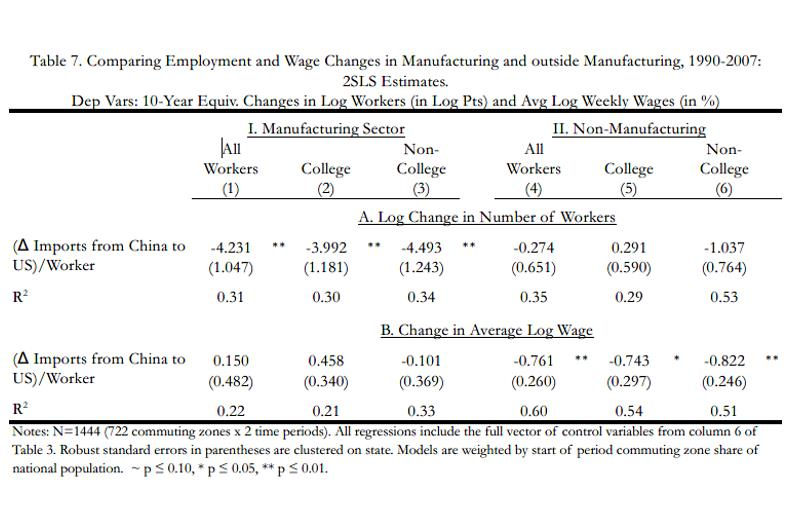
\includegraphics{figures/table7.jpg}
		}
		%\includegraphics[scale=1.0]{figurefile}
		%\caption{Fig1}
%		\label{fig:campus}
	\end{figure}
\end{frame}



\subsection{Public transfer payment}
\begin{frame}{Public transfer payment}
	\begin{figure}[thpb]
		\centering
		\resizebox{1\linewidth}{!}{
			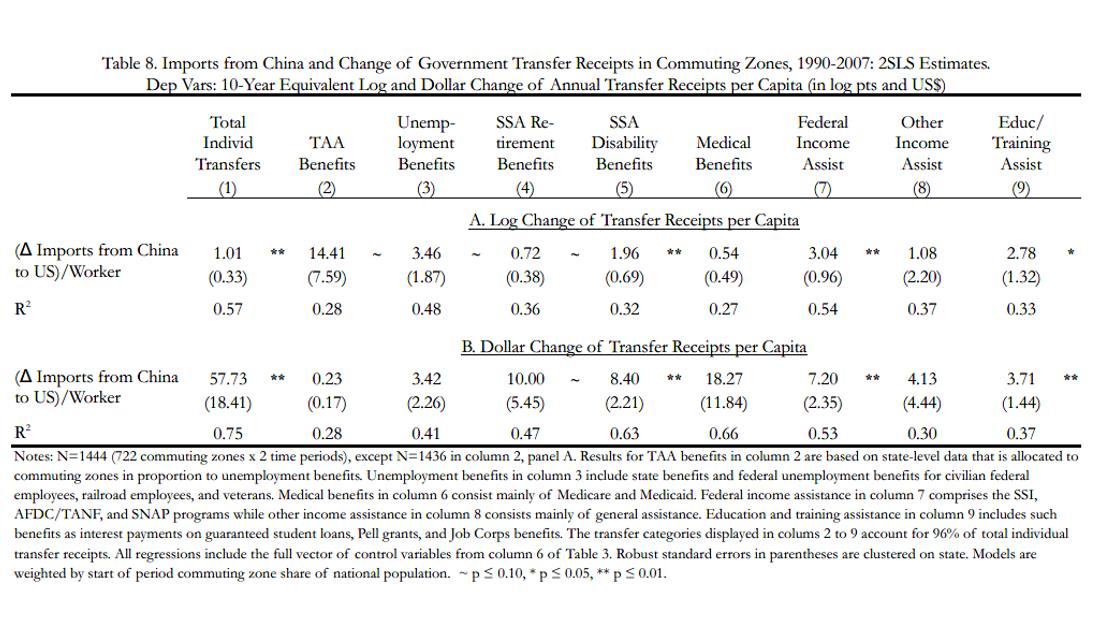
\includegraphics{figures/table8.jpg}
		}
		%\includegraphics[scale=1.0]{figurefile}
		%\caption{Fig1}
%		\label{fig:campus}
	\end{figure}
\end{frame}


\subsection{Household income}
\begin{frame}{Household income}
	\begin{figure}[thpb]
		\centering
		\resizebox{1\linewidth}{!}{
			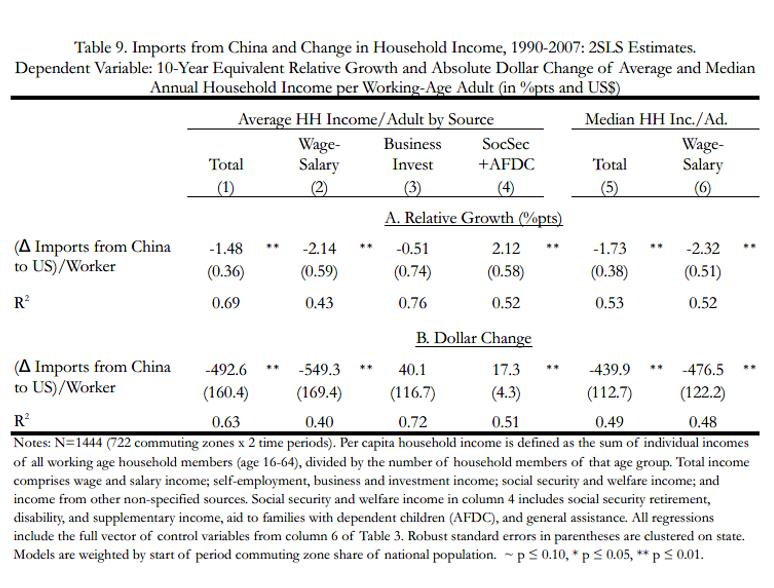
\includegraphics{figures/table9.jpg}
		}
		%\includegraphics[scale=1.0]{figurefile}
		%\caption{Fig1}
%		\label{fig:campus}
	\end{figure}
\end{frame}

\subsection{Robustness check}
\begin{frame}{Robustness check}
	(1)modify the definition of exposure——China's growth not only displaces U.S. producers in the U.S. market but may also affect U.S. sales in the foreign markets that U.S. industries serve.
	 		
		\begin{center}		
			\LARGE $\sum_{j} \frac{E_{ijt}}{E_{ujt}} \frac{\Delta M_{ucjt} + \sum_{o \neq c} \frac{X_{oujt}}{X_{ojt} \Delta M_{ocjt} } }{E_{it}} $
		\end{center}
	.\\
	(2)Exposure to final Goods and Intermediate Inputs——using total China imports per worker less China imports of intermediate inputs per worker
\end{frame}

\begin{frame}{Robustness check}


(3)Net Chinese Imports per Worker
\begin{center}		
	\LARGE $\sum_{j} \frac{E_{ijt}}{E_{ujt}} \frac{\Delta M_{ucjt} } {E_{it}} - \sum_{j} \frac{E_{ijt}}{E_{ujt}} \frac{\Delta X_{cujt} } {E_{it}} $
\end{center}
(4)An alternative to studying net import effects——use the gravity-based approach to measure the exposure\\  . \\
(5)Use the factor content of U.S. net imports from China to replace imports per worker
\begin{center}		
	\LARGE $\sum_{j} \frac{E_{ijt}}{E_{ujt}} \frac{\tilde{E}_{uj0}}{V_{uj0}} \frac{\Delta M_{ucjt} } {E_{it}} - \sum_{j} \frac{E_{ijt}}{E_{ujt}} \frac{\tilde{E}_{uj0}}{V_{uj0}} \frac{\Delta X_{cujt} } {E_{it}} $
\end{center}
\end{frame}






\begin{frame}{Robustness check}
	\begin{figure}[thpb]
		\centering
		\resizebox{1\linewidth}{!}{
			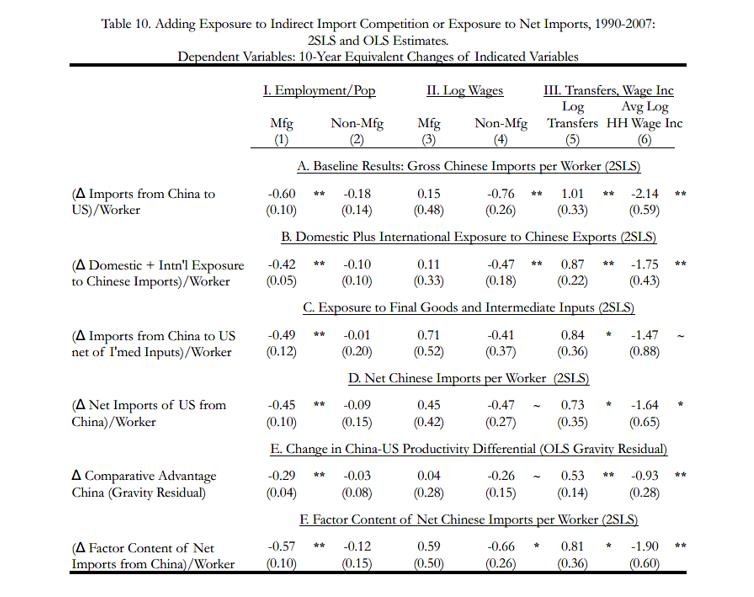
\includegraphics{figures/table10.jpg}
		}
		%\includegraphics[scale=1.0]{figurefile}
		%\caption{Fig1}
		%		\label{fig:campus}
	\end{figure}
\end{frame}


\section{Conclusion}
\begin{frame}{Conclusion}  %将来可做的方向
	\begin{itemize}
	\item<0->  The EXPOSURE to Chinese import competition affects US local labor markets
	\item<0->  The rising EXPOSURE increase unemployment, lowers labor force participation and reduces wages in local labor market.
	\item<0->  This effect explains 1/4 of the contemporaneous aggregate decline in U.S. manufacturing employment.
\end{itemize}
\end{frame}

\begin{frame}{Thank you}
\begin{center}
\begin{minipage}{1\textwidth}
	\setbeamercolor{mybox}{fg=white, bg=black!50!blue}
 \begin{beamercolorbox}[wd=0.70\textwidth, rounded=true, shadow=true]{mybox}
\LARGE \centering Thank you for listening!  %结束语
\end{beamercolorbox}
 \end{minipage}
\end{center}
\end{frame}

\begin{frame}{Q\&A}
\begin{center}
	\begin{minipage}{1\textwidth}
		\setbeamercolor{mybox}{fg=white, bg=black!50!blue}
		\begin{beamercolorbox}[wd=0.70\textwidth, rounded=true, shadow=true]{mybox}
			\LARGE \centering  Questions?  %请求提问
		\end{beamercolorbox}
	\end{minipage}
\end{center}
\end{frame}

% -----------------------------------------------------------------------------
\end{document}
%文档结束




%\begin{frame}{Background}
%	\begin{columns}[T] % align columns
%		\begin{column}<0->{.40\textwidth}
%			\begin{figure}[thpb]
%				\centering
%				\resizebox{1\linewidth}{!}{
%					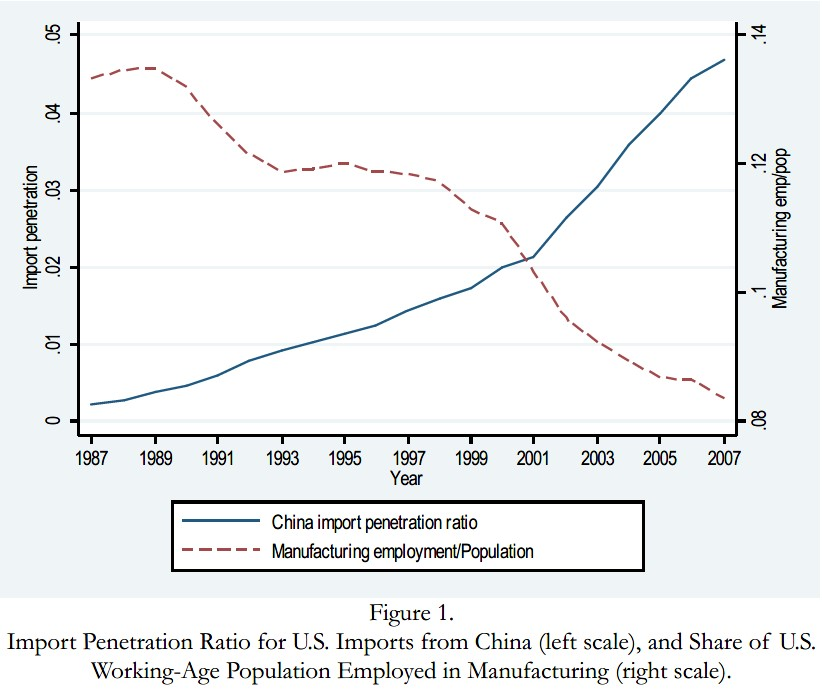
\includegraphics{figures/fig1.jpg}
%				}
%				%\includegraphics[scale=1.0]{figurefile}
%				\caption{SUSTech Campus}
%				\label{fig:campus}
%			\end{figure}
%		\end{column}%
%		\hfill%
%		\begin{column}<0->{.65\textwidth}
%			\begin{itemize}
%				\item<1-> 短信息(SMS)成为现代通讯的重要组成部分
%				\begin{itemize}
%					\item<1-> 很多组织或网站使用短信息作为身份验证的辅助通道
%				\end{itemize}
%				\item<2-> 现代短消息的发送,在抵达终端之前不接触蜂窝网络
%				\begin{itemize}
%					\item<2-> 短信息(SMS)成为现代通讯的重要组成部分
%				\end{itemize}
%			\end{itemize}
%		\end{column}%
%	\end{columns}
%\end{frame}





% \begin{frame}
%	\frametitle{OTT服务}
%	\begin{figure}[!t]
%		\centering
%		\includegraphics[width=2in]{figures/sustech.pdf}
%		\caption{OTT服务}
%		\label{figure3_OTT}
%	\end{figure}
%	\begin{center}
%		OTT服务支持在数据网络上提供短信和语音等第三方服务。\\
%		OTT可以使用云服务来存储和同步SMS到用户的其他设备。
%	\end{center}
	
%\end{frame}